\chapter{Background}\label{chap:background}



\section{Transformers}

The Transformer, introduced by Vaswani et al. in 2017 \cite{vaswani2017attention}, revolutionized sequence-to-sequence tasks in Natural Language Processing(NLP). This architecture overcame limitations of traditional methods like LSTM and gated RNNs \cite{hochreiter1997long}\cite{chung2014empirical} by harnessing self-attention mechanisms. Self-attention enabled parallel computation, addressing slow training and capturing long-range dependencies. Following the success of Transformer in NLP, Vision Transformer (ViT) was introduced by Dosovitskiy et al. \cite{dosovitskiy2020image} as an alternative to Convolutional Neural Networks (CNNs) for image recognition.\\
This section explores the fundamental components of the Transformer: self-attention, multi-head attention, positional encoding, and feed-forward networks. This section describes the Transformer block utilized within GroupViT, for both textual and visual backbone. A firm understanding of the Transformer is essential to comprehending the functioning of GroupViT.

\subsubsection{Input Tokens}
In natural language processing (NLP) and vision transformers (ViT), tokens play a crucial role in representing discrete units within an input sequence or image. Tokens can be individual words, subwords, or even characters, depending on the tokenization strategy employed.
Tokenization is the process of breaking down a text or image into these discrete tokens. For text data, popular tokenization methods include Byte-Pair Encoding (BPE) and WordPiece\cite{gage1994new}\cite{wu2016google}. BPE and WordPiece algorithms split text into subword tokens, enabling more flexible handling of languages with complex word structures. Each token is then mapped to an embedding vector using an embedding layer. These embedding vectors capture the semantic meaning and contextual information of the tokens within the text.
In the case of ViT (Vision Transformers), images are divided into non-overlapping patches, and each patch is treated as a token \cite{dosovitskiy2020image}. These image patch tokens are then converted into embeddings using linear projections. This approach allows ViT models to process and understand images in a manner similar to how traditional transformer models handle text data.
\subsubsection{Positional Encoding}

Positional Encoding is crucial for maintaining token order in Transformer models. Often implemented with sinusoidal functions across various frequency dimensions, it enhance the model's grasp of sequential patterns. It is worth noting that ViT employs positional embeddings differently from NLP. In ViT, these embeddings encode the spatial locations of image patches. As a result, they are added to patch embeddings, enabling ViT to capture spatial relationships and contextual information. GroupViT employs simple positional embeddings for its visual and text encoders.

\subsection{Attention}
Attention is a mechanism in the neural network that a model can learn to make predictions by selectively attending to a given set of data. The amount of attention is quantified by learned weights and thus the output is usually formed as a weighted average\cite{weng2020transformer}.
% In the realm of transformer models, the concept of attention is foundational. It serves to compute the significance or relevance of elements within a sequence. 
For each element, distinct query, key, and value representations are computed. Attention scores are derived from dot products between queries and keys, and they are adjusted by a normalization factor. The application of a softmax function further refines these scores, resulting in attention weights. These weights play a crucial role in shaping the attended representations obtained by applying them to the value vectors

Furthermore, this attention mechanism takes on two key forms: self-attention and cross-attention. Self-attention emerges when the attention source (query) aligns with the attention target (keys and values) within the same sequence. In contrast, cross-attention comes into play when the attention source differs from the attention target.

Assuming learnable weight matrices \(W_f\), \(W_q\), \(W_k\), and \(W_v\) in \(\mathbb{R}^{D \times D}\):
\begin{equation}
    \text{Attention\_Matrix}(q, k) = \text{Softmax}\left(\frac{qW_q(kW_k^T)}{\sqrt{D}}\right)
\end{equation}
\begin{equation}
\label{eq:attn}
    \text{Attention}(q, k) = \left(\text{Attention\_Matrix}(q, k) \cdot vW_v\right)W_f
\end{equation}
% Within the attention mechanism, a significant distinction arises between self-attention and cross-attention. Self-attention occurs when the source of attention (denoted as \(q\)) coincides with the focus of attention (referred to as \(k\)) within the same sequence. In contrast, cross-attention comes into play when \(q\) and \(k\) represent distinct entities.

Mathematically, this differentiation can be succinctly described as follows:

\begin{equation}
    \text{Attention}(q, k) = 
    \begin{cases}
        \text{Self-attention}: & \text{Attention}(q, q) \quad \text{(when \(q = k\))} \\
        \text{Cross-attention}: & \text{Attention}(q, k) \quad \text{(when \(q \neq k\))}
    \end{cases}
\end{equation}

\subsection{Multi-Head Attention}
To enhance expressiveness and capture intricate patterns, Transformers often incorporate the concept of multi-head attention. In this mechanism, several sets of learnable weight matrices for queries, keys, and values are utilized. We define these learnable weights for each head as \(W^{(i)}_q\), \(W^{(i)}_k\), \(W^{(i)}_v\) in \(\mathbb{R}^{D \times D_h}\), where \(D\) represents the model dimension, \(i\) indexes the individual attention head, and \(D_h\) represents the dimension focused on by each head. \(D_h\) is obtained by dividing \(D\) into \(H\) chunks equally, where \(H\) is the number of heads.

Mathematically, the multi-head attention process can be expressed as follows:

\begin{equation}
\text{MultiHeadAttnMat}(q, k, i) = \text{Softmax}\left(\frac{qW_{q}^{(i)}(kW_{k}^{(i)})^{T}}{\sqrt{D}}\right)
\end{equation}
\begin{equation}
\text{$Attn_{h}$}(q, k, i) = \text{MultiHeadAttnMat}(q, k, i)(vW_{v}^{(i)})
\end{equation}

The outputs of the different attention heads are subsequently concatenated and linearly transformed by the projection weight \(W_f \in \mathbb{R}^{D \times D}\), resulting in the final output. 
% \begin{equation}
% \label{eq:multiheadattn}
% \text{MultiHeadAttention}(q, k) = \text{Concat}\(\text{$Attn_h$}(q, k, i)\)W_{f}
% \end{equation}
% \begin{equation}
% \label{eq:multiheadattn}
% \text{MSA}(q, k) = \left(\text{Concat}_{i=0}^{H-1} \text{$Attn_h$}(q, k, i)\right)W_{f}
% \end{equation}
\begin{equation}
\label{eq:multiheadattn}
\text{MSA}(q, k) =  \text{[$Attn_{0}(q, k, i), ... Attn_{H-1}(q, k, i)$ ]}W_{f}
\end{equation}

This strategic combination empowers the model to simultaneously attend to various aspects or relationships within the image. Consequently, a more nuanced representation of the interdependencies between image patches is obtained.



\subsection{ Feed-forward Networks}
The Transformer model incorporates feed-forward neural networks to process the output from the self-attention mechanism. These networks consist of two linear layers with a GeLU activation function in between\cite{hendrycks2016gaussian}. By incorporating non-linear transformations, the feed-forward networks enable the model to capture complex relationships within the sequence effectively.
\begin{equation}
\label{eq:mlp}
\text{MLP}(x) = \text{GELU}(xW_1 + b_1)W_2 + b_2
\end{equation}


\subsection{Transformer block}
In Chapter \ref{chap:approach}, GroupViT employs a term called the `Transformer block' which is an alternative term to the `Transformer encoder' in the original work by Vaswani et al. \cite{vaswani2017attention} and in Dosovitskiy et al.'s Vision Transformer (ViT) \cite{dosovitskiy2020image}. This section delves into a detailed explanation of this fundamental building block.

The Transformer block consists of alternating layers of multi-headed self-attention (MSA) as shown in Eq. \ref{eq:multiheadattn} and MLP blocks as shown in Eq. \ref{eq:mlp}. Layernorm (LN) \cite{qiao2019micro} is applied before every block, and residual connections \cite{baevski2018adaptive} after every block as shown from Eq. \ref{eq:block} to Eq. \ref{eq:finalpass}, where \(x\) represents the input to the Transformer block and 
% \(x'\) is the result after applying Multi-Head Self-Attention (MSA) to the input.
% \(x'\) is the output of the Multi-Layer Perceptron (MLP) transformation.
\(y\) is the final output of the Transformer block after Layer Normalization (LN).
\begin{align}
\label{eq:block}
\text{Multi-Head Self-Attention (MSA):} \quad x' &= \text{MSA}(\text{LN}(x)) + x \\
\label{eq:mlppass}
\text{Multi-Layer Perceptron (MLP):} \quad x' &= \text{MLP}(\text{LN}(x')) + x' \\
\label{eq:finalpass}
\text{Layer Normalization (LN) and Output:} \quad y &= \text{LN}(x') \quad \text{(final output)}
\end{align}

In the upcoming chapter, we will harness the capabilities of this Transformer block within the GroupViT framework. Our focus will be twofold: firstly, using it to generate image patch embeddings within the visual backbone, and secondly, utilizing it as the text encoder for generating text embeddings within the GroupViT architecture.
% Multi-Head Self-Attention (MSA):
% \begin{equation}
% \label{eq:msapass}
% x' = \text{MSA}(\text{LN}(x)) + x
% \end{equation}

% Multi-Layer Perceptron (MLP):
% \begin{equation}
% \label{eq:mlppass}
% x' = \text{MLP}(\text{LN}(x')) + x'
% \end{equation}

% Layer Normalization (LN) and Output:
% \begin{equation}
% \label{eq:finalpass}
% y = \text{LN}(x')    \quad \text{(final output)}
% \end{equation}



\begin{figure*}
  \centering
  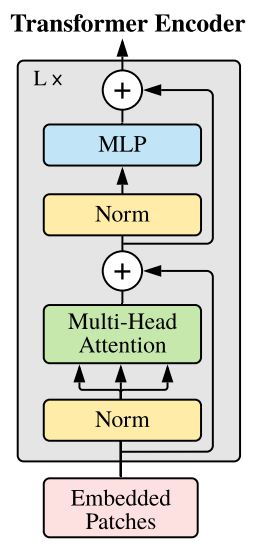
\includegraphics[width=0.3\textwidth]{figures/experiments/figures/transformerblock.png}
  \caption[\textbf{Architecture of Transformer Block}]{\textbf{Architecture of Transformer Block}. This illustration of the Transformer encoder is present in ViT \cite{dosovitskiy2020image}.}
  \label{fig:inf}
\end{figure*}

\section{DINO}
The self-supervised model DINO, introduced by Caron, Mathilde, et al. \cite{caron2021emerging}, demonstrates performance comparable to many state of the art convolutional networks (convnets) trained in supervised manner. Notably, the features extracted from DINO reveal explicit information about the semantic segmentation of images and scene layout. This characteristic stands out in comparison to supervised Vision Transformers (ViTs) and convnets. It's noteworthy that this ability could have valuable applications for weakly supervised image segmentation.
\subsection{Knowledge distillation}
Central to DINO is the concept of knowledge distillation. It involves a student network predicting the teacher network's output. The teacher network is constructed using a momentum encoder, as shown in Figure \ref{fig:dino}. The optimization objective is to minimize the cross-entropy loss between the probability distributions generated by the teacher ($P_t(x)$) and student ($P_s(x)$) networks, as expressed in Equation \ref{eq:dino_objective}.
\begin{equation}
\label{eq:dino_objective}
\min_{\theta_s} \mathcal{H}(P_t(x), P_s(x))
\end{equation}
Here, `min \( \theta_s \)' signifies adjusting the student network's parameters \( \theta_s \) during training. The term \( \mathcal{H}(P_t(x), P_s(x)) \) represents the cross-entropy loss between the predicted probability distributions. This optimization aligns student and teacher predictions, transferring knowledge effectively.

\subsection{Multi-crop strategy}
DINO generates multiple crops of an image, naturally having diverse perspective, represented as a set $\mathcal{V}$ encompassing various views, including both global views ($x_{g1}$ and $x_{g2}$). While all crops are processed by the student network, only the global views undergo evaluation by the teacher network. This approach facilitates the establishment of connections that span from local to global features. To go into specific of the Eq. \ref{eq:dino_objective} mentioned above, we provide Eq. \ref{eq:dino_loss}
\begin{equation}
\label{eq:dino_loss}
\min_{\theta_s} \sum_{x \in \{x_{g1},x_{g2}\}} \sum_{x_0 \in \mathcal{V}, x_0 \neq x} H(P_t(x), P_s(x_0))
\end{equation}
Here, $H(P_t(x),P_s(x_0))$ denotes the cross-entropy loss between the probability distributions $P_t(x)$  and $P_s(x_0)$, $x$ and $x_0$ represent input images from the set $\mathcal{V}$, and the goal is to minimize the disparity between predictions made by the student and teacher networks. 


\begin{figure*}
  \centering
  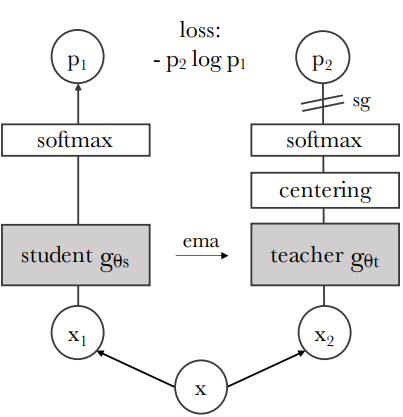
\includegraphics[width=0.3\textwidth]{figures/experiments/figures/dino.png}
  \caption[\textbf{DINO Architecture }]{\textbf{Architecture of DINO}. DINO is illustrated in the case of one single pair of views (x1, x2) for simplicity. The
model passes two different random transformations of an input
image to the student and teacher networks. Both networks have
the same architecture but different parameters. The output of the
teacher network is centered with a mean computed over the batch.
Each networks outputs a K dimensional feature that is normalized
with a temperature softmax over the feature dimension. Their
similarity is then measured with a cross-entropy loss. We apply a
stop-gradient (sg) operator on the teacher to propagate gradients
only through the student. The teacher parameters are updated with
an exponential moving average (ema) of the student parameters. Illustration provided in 
\cite{caron2021emerging}.}
  \label{fig:dino}
\end{figure*}
\subsection{Momemtum Encoder}
To train the teacher network \( g_{\theta_t} \), DINO employs an exponential moving average (EMA) on student weights using a momentum encoder \cite{caron2021emerging}. The update rule is given by Equation \ref{eq:dinome}.
\begin{equation}
\label{eq:dinome}
\theta_t \leftarrow \lambda\theta_t + (1 - \lambda)\theta_s
\end{equation}
Furthermore, DINO applies centering and sharpening of the momentum teacher outputs to prevent model collapse. Centering prevents one dimension from dominating and encourages uniform distribution, while sharpening has the opposite effect. By balancing these operations, DINO maintains stability while avoiding collapse.\\
In this work, we explore ways to utilize features extracted from DINO to boost visual grouping in GroupViT.

% The MLP-Mixer is a neural architecture introduced in the paper "MLP-Mixer: An all-MLP Architecture for Vision" by Ilya Tolstikhin et al. in 2021. It presents an alternative approach to convolutional neural networks (CNNs) and transformer-based models for visual tasks. In the context of GroupViT, the term "MLP-Mixer" refers to a specific component or technique used to handle the variance in the number of group tokens in the second stage of the GroupViT architecture. The MLP-Mixer likely involves the use of multi-layer perceptrons (MLPs) to process and combine the group token embeddings, allowing for the integration of different token counts efficiently.


% Sublayers utilize residual connections and normalization:
% \begin{equation}
%     \text{Sublayer}(Layer, x) = \text{LayerNorm}(Layer(x) + x)
% \end{equation}
% \begin{equation}
%     \text{Sublayer}(Layer, y, x) = \text{LayerNorm}(Layer(y, x) + y)
% \end{equation}

% The self-attention transformer layer, defined as \(\text{TransformerAtn}(x)\), involves sublayers for multi-head self-attention and point-wise feed-forward networks, as introduced by Vaswani et al. \cite{vaswani2017attention}:
% \begin{equation}
%     \text{TransformerAtn}(x) = \text{Sublayer}(\text{MultiHeadSelfAttention}, x)
% \end{equation}
% \begin{equation}
%     \text{TransformerLayer}(x) = \text{Sublayer}(\text{FFN}, \text{TransformerAtn}(x))
% \end{equation}

% The output shape remains the same as the input \(x\).



